\documentclass[11pt]{beamer} % Определяем тип документа как презентацию
% в квадратных скобках размер шрифта: 8pt, 9, 10, 11 (def), 12, 14, 17, 20.

% Общее:
\usetheme{CambridgeUS} % колонтитулы, углы, и другая красота
% Другие темы можно найти на https://latex-beamer.com/tutorials/beamer-themes/
\usecolortheme{seahorse} % но по факту мы почти все цвета сами задаем
% https://deic.uab.cat/~iblanes/beamer_gallery/index_by_color.html
\usefonttheme{professionalfonts}

\usepackage {mathtools} % красивая математика
\usepackage{amsmath,amsfonts,amssymb,amsthm,mathtools} % еще математика

\usepackage[
backend=biber,
style=numeric,
sorting=nty
]{biblatex} % для библиографии
\addbibresource{references.bib}
\usepackage{hyperref} % для ссылок
\usepackage{epigraph}
\usepackage{graphicx}

% Создаем цвета
\definecolor{darkredNES}{RGB}{115,15,15} % тёмно-красный
\definecolor{darkblueNES}{RGB}{20,20,100} % тёмно-синий
\definecolor{redNES}{RGB}{170,35,35} % красный посветлее
\definecolor{darkgreenNES}{RGB}{7,110,7} % тёмно-зеленый
\definecolor{alertredNES}{RGB}{125,25,25} % красный средний
% Однако в основном проще пользоваться стандартными цветами, подробнее тут:
% https://www.overleaf.com/learn/latex/Using_colours_in_LaTeX

\setbeamercolor*{palette primary}{bg=darkblueNES} %правые рамки
\setbeamercolor*{palette secondary}{bg=darkblueNES, fg = white} %центральные
\setbeamercolor*{palette tertiary}{bg=darkblueNES, fg = white} %левые

\setbeamercolor*{titlelike}{bg=darkblueNES} % названия слайдов
\setbeamercolor*{title}{bg=darkblueNES, fg = white} % титул и отделы
\setbeamercolor*{item}{fg=redNES} % для списков (например, в оглавлении)
\setbeamercolor*{caption name}{fg=darkblueNES} % названия картинок
\setbeamercolor{alerted text}{fg=alertredNES} % выделенка

\setbeamertemplate{blocks}[rounded, shadow=true]
\setbeamercolor{block title}{bg=darkblueNES, fg=white}
\setbeamercolor{block title alerted}{bg=alertredNES, fg=white}
\setbeamercolor{block title example}{bg=darkgreenNES, fg=white}

\setbeamercolor{bibliography entry author}{fg=black}
\setbeamercolor{bibliography entry title}{fg=black}
\setbeamercolor{bibliography entry note}{fg=darkblueNES}

\setbeamercolor{page number in head/foot}{fg=white}

% Для русского нам пригодится
\usepackage[english]{babel} % локализация и переносы
\usepackage{fontspec}
\usepackage[T2A]{fontenc} % кодировка
\usepackage[utf8]{inputenc} % кодировка исходного текста
\usepackage{cmap} % поиск в PDF
\usepackage{mathtext} % русские буквы в формулах

% Шрифты
\setsansfont{Times New Roman} % Настройка Шрифта
% \setsansfont{Noto Sans} этот можете использовать, если вам не нравятся засечки на буквах
% \setmainfont{Arial} % Дополнительно
% \setmonofont{Arial} % Нужно Разобраться за что они отвечают
% Другие шрифты можно поскачивать на https://www.ctan.org/tex-archive/fonts

% Работа с картинками
\usepackage{graphicx} % Для вставки рисунков
\setlength\fboxsep{3pt} % Отступ рамки \fbox{} от рисунка
\setlength\fboxrule{1pt} % Толщина линий рамки \fbox{}
\usepackage{wrapfig} % Обтекание рисунков текстом
\DeclareGraphicsExtensions{.pdf,.png,.jpg,.HEIC} % работа с форматами
% \graphicspath{{images/}} % папки с картинками, в оверлифе это не нужно
% Ещё о картинках https://www.overleaf.com/learn/latex/Inserting_Images

% Работа с таблицами
\usepackage{array,tabularx,tabulary,booktabs} % Дополнительное для таблиц
\usepackage{longtable} % Длинные таблицы
\usepackage{multirow} % Слияние строк в таблице

% Свои команды, если лень прописывать \mathbb итп.
\def\E{\exists} % существует
\def\A{\forall} % для всех

\def\La{\mathcal{L}} % калиграфическое L (Лагранжиан, преобразования Лапласа)
\def\la{\lambda} % лямбда
\def\a{\alpha} % альфа
\def\b{\beta} % бэта
\def\e{\varepsilon} % эпсилон (покрасивее)
\let\phi\varphi % фи (покрасивее)

\def\N{\mathbb{N}} % натуральные
\def\Z{\ensuremath{\mathbb{Z}}} % целые
\def\R{\mathbb{R}} % рациональные
\def\C{\mathbb{C}} % комплексные

\def\~{\sim} % подобно

%Возможно, у вас возникнут проблемы с буквой @, попробуйте одно из следующих:
%\makealetter
%\makeatother 
% В преамбуле можно сделать небольшие изменения (цвет, шрифт итд.) Если есть желание изменить больше, возможно, проще выбрать другой шаблон.

%Логотип
\titlegraphic{
\includegraphics[height=1.9cm]{images/mipt_logo.png}}

%Размеры шрифтов титульного листа; Цвета определены в преамбуле
\setbeamerfont{title}{size=\huge}
\setbeamerfont{subtitle}{size=\large}
\setbeamerfont{author}{size=\normalsize}
\setbeamerfont{date}{size=\normalsize}
\setbeamerfont{institute}{size=\normalsize}
% Больше о шрифтах вы найдете в том числе по следующей ссылке:
% https://tex.stackexchange.com/questions/183052/what-are-all-the-possible-first-arguments-to-setbeamerfont

%Тут квадратные скобки --- всё, что будет внизу странички
\title[ФРКТ, МФТИ]{Работа 4.3.1}
\subtitle{Изучение дифракции света}
\author[Тихонов Д.Р., Казачков А.Н.]{}
\institute[]{Московский физико-технический институт \\ Физтех-школа Радиотехники и Компьютерных Технологий}
\date[\textcolor{white}{19 февраля 2024 г.}]{19 февраля 2024 г.}



% Следующее пригодится, если нужно показывать начало секции с оглавлением
%\AtBeginSection[]
%{
%  \begin{frame}
%    \frametitle{Contents}
%    \tableofcontents[currentsection]
%  \end{frame}
%}

% \AtBeginSection[]{
%   \begin{frame}
%   \vfill
%   \centering
%   \begin{beamercolorbox}[sep=8pt,center,shadow=true,rounded=true]{title}
%     \usebeamerfont{title}\insertsectionhead\par%
%   \end{beamercolorbox}
%   \vfill
%   \end{frame}
% }

\addto\captionsenglish{\renewcommand{\figurename}{Рисунок}}

\begin{document}

\frame{\titlepage}

\begin{frame}
    \frametitle{Содержание работы}
    \tableofcontents
\end{frame}

% % Далее начнем работу со слайдами:
\section{Цели работы}
    \begin{frame}{Цели работы}
        \begin{itemize}
            \item изучить свойства голограммы точечного источника:
            \begin{itemize}
                \item изучить \textit{зонную решётку Габора} (голограмма точечного источника)
            \end{itemize}

            \item изучить свойства голограммы объёмного источника:
            \begin{itemize}
                \item оценить угол падения опорной волны, который был выбран при создании голограммы
                \item убедиться, что изображение предмета восстанавливается по небольшой части голограммы
                \item проследить за изменением масштабов изображений при освещении голограммы сферической волной
            \end{itemize}
        \end{itemize}
    \end{frame}

    \section{Оборудование}
    \begin{frame}{Оборудование}
        \begin{itemize}
            \item гелий-неоновый лазер
            \item голограммы
            \item набор линз
            \item предметная шкала
            \item экран
            \item линейка
        \end{itemize}
    \end{frame}

    \section{Теоретические сведения}

   \begin{frame}{Теория. Голография и голограмма}
        % \begin{itemize}
            \textit{Голограмма} -- фотопластинка с зарегистрированным на ней результатом интерференции предметной и опорной волны. \\
            \textit{Голография} -- способ записи изображения, который позволяет по картине интенсивности восстановить полную информацию о волновом поле. 
        % \end{itemize}
        \begin{columns}[T]
            \begin{column}{0.5\textwidth}
                \centering
                \begin{figure}
                    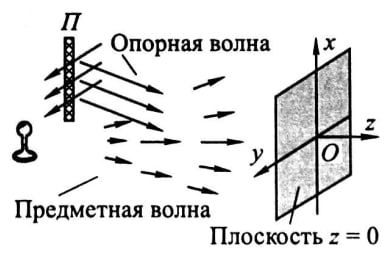
\includegraphics[width=\textwidth]{images/hologram_holography.jpg}
                    \caption{Запись голограммы}
                    \label{hol_hol}
                \end{figure}
            \end{column}
    
            \begin{column}{0.5\textwidth}
                \begin{itemize}
                    \item \textit{Предметная волна} -- волна, падающая на фотопластинку после отражения от предмета
                    \item \textit{Опорная волна} -- волна, падающая сразу на фотопластинку
                \end{itemize}
            \end{column}
        \end{columns}       
   \end{frame}

   \begin{frame}{Теория. Характеристика волн}
        \textbf{Когерентность} предметной и опорной волн обеспечивается высокой степенью монохроматичности лазерного излучения.\\
        Функция пропускания фотопластинки:
        \begin{equation}
           t(x,y) \propto I(x,y) = |f_{\text{п}}(x,y) + f_{\text{о}}(x,y)|^2 = a^2+a_о^2+2 a a_o \cos (\varphi - \varphi_о),
        \end{equation}
        т.е. сохранилась информация о фазе предметной волны $\phi(x,y)$, где $(x,y)$ -- точка в плоскости $z=0$.
   \end{frame}

    \begin{frame}{Теория. Точечный источник. Запись голограммы}
    \begin{columns}
        \column{0.4\textwidth}
            \begin{figure}[H]
                \centering
                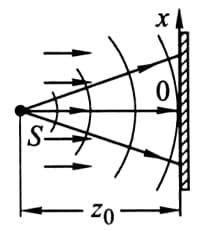
\includegraphics[width = 0.7\textwidth]{images/photo_processing.jpg}
                \caption{Запись голограммы}
            \end{figure}
        
        \column{0.6\textwidth}
            \begin{itemize}
               \item Положим нулевой фазу колебаний в плоскости $z = 0$ 
               \item Для опорной волны $f_0 = a$
               \item Для предметной волны амплитуда сферической волны $\approx$ амплитуде плоской волны $f_\text{п} = \frac{a_\text{п}}{r}e^{ikr} \approx ae^{ikr}$
               \item $r = \sqrt{z_0^2 + x^2 + y^2}$ -- расстояние от источника S до точки $(x,y)$ на фотопластинке
               \item Суммарное поле на фотопластинке $f = ae^{ikr} + a$
               \item Функция пропускания: $t(x, y) \propto \left| a+ a e^{i k r}\right|^2$
           \end{itemize}
        \end{columns}       
   \end{frame}

    \begin{frame}{Теория. Точечный источник. Восстановление голограммы}
        \begin{columns}
        \column{0.5\textwidth}
            \begin{figure}[H]
                \centering
                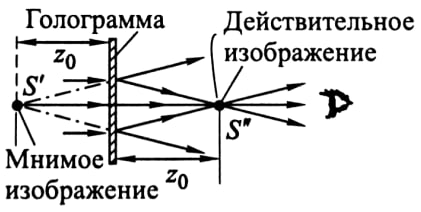
\includegraphics[width = 0.9\textwidth]{images/recovery.jpg}
                \caption{Восстановление голограммы}
            \end{figure}
        
        \column{0.5\textwidth}
            \begin{itemize}
               \item Освещаем голограмму плоской нормально падающей волной (\textit{восстанавливающей})
               \item Для упрощения положим $f_{-}(x,y) = 1$ (фаза $= 0$, амплитуда $= 1$)   
           \end{itemize}
        \end{columns}
       \begin{equation}
           f_+ (x, y) = \left| a+ a e^{i k r}\right|^2 = 2 a^2 (1+\cos (k r)) = 2 a^2 + a^2 e^{i k r} +a^2 e^{- i k r}
       \end{equation}
       Структура полученной волны: суперпозиция плоской и двух сферических волн.
   \end{frame}

   \begin{frame}{Теория. Зонная решётка Габора}
        \textbf{Зонная решётка Габора} -- это особая интерференционная картина, соответствующая голограмме точечного источника.
        \begin{columns}
            \column{0.3\textwidth}
                \begin{figure}[H]
                    \centering
                    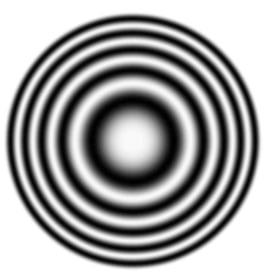
\includegraphics[width = \textwidth]{images/Gabor_grating.jpg}
                    \caption{Зонная решётка Габора}
                    \label{fig:Gabor}
                \end{figure}
            
            \column{0.7\textwidth}
                \begin{itemize}
                   \item Голограмма точечного источника имеет вид колец (рис. \ref{fig:Gabor}) с радиусами
                    \begin{equation*}\label{key}
                    	\rho_m = \sqrt{m \lambda z_0},
                    \end{equation*}
                    где нечётному $ m $ соответствуют тёмные кольца.  
               \end{itemize}
        \end{columns}
   \end{frame}

   \begin{frame}{Теория. Разрешающая способность голограммы}
        Голограмма создаёт изображение — дифракционное пятно, размер которого определяется формулой \cite{lab}:
        \begin{equation}
            \Delta x \sim \frac{\lambda}{D} z_0,
        \end{equation}
        \begin{itemize}
            \item $z_0$ -- расстояние от точечного источника до голограммы в процессе записи
            \item $D$ -- размер голограммы
            \item $\lambda$ -- длина волны
        \end{itemize}
       
   \end{frame}
    
    \section{Экспериментальная установка}

    \begin{frame}{Схема экспериментальной установки}
    \small
    \begin{figure}[H]
        \centering
        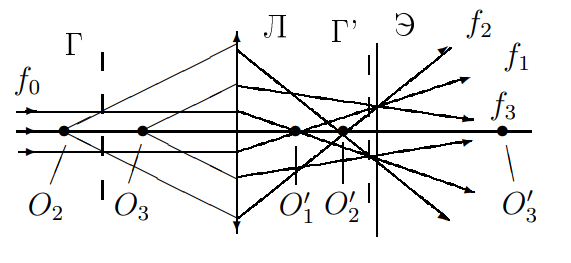
\includegraphics[width = 0.8\textwidth]{images/installation.png}
        \caption{Схема установки. Г -- голограмма точечного источника}
        \label{fig:installation_1}
    \end{figure}
    \end{frame}

    \section{Изучение характеристик голограммы точечного источника}

    \begin{frame}{Настройка установки. Определение цены деления предметной шкалы}
    \small
        \begin{columns}
        \column{0.5\textwidth}
            \begin{figure}[H]
                \centering
                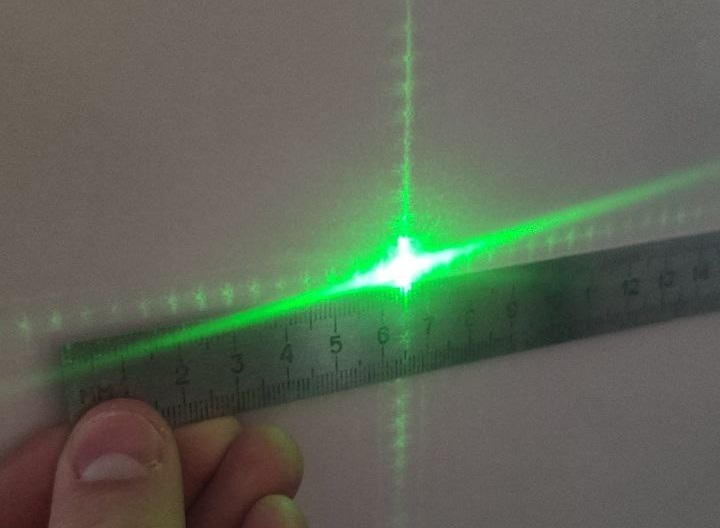
\includegraphics[width = \textwidth]{images/cross_subject_scale.jpeg}
                \caption{Дифракционная картина, созданная крестообразной шкалой}
            \end{figure}
        
        \column{0.5\textwidth}
            \begin{itemize}
                \item $\Delta x = \left( 4.4 \pm 0.1 \right) \text{ мм}$ -- расстояние между дифракционными максимумами
                \item $\frac{\lambda}{D} = \frac{\Delta x}{L} \Rightarrow D = \frac{\lambda L}{\delta X} = \left( 0.104 \pm 0.003 \right) \text{ мм}$ -- цена деления предметной шкалы
            \end{itemize}
        
        \end{columns}
    \end{frame}

    \begin{frame}{Настройка установки. Определение цены деления предметной шкалы}
    \small
        \begin{columns}
        \column{0.5\textwidth}
            \begin{figure}[H]
                \centering
                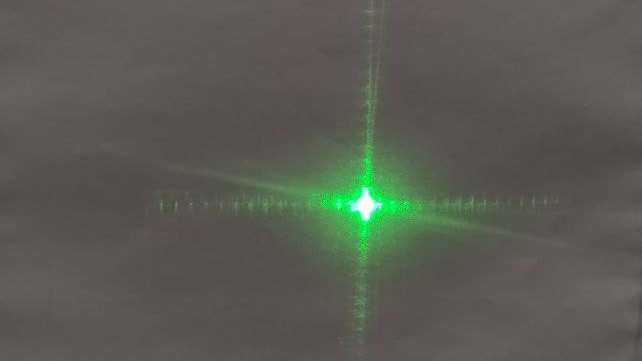
\includegraphics[width = \textwidth]{images/increased_cross_subject_scale.jpg}
                \caption{Увеличенное изображение предметной шкалы}
            \end{figure}
        
        \column{0.5\textwidth}
            \begin{itemize}
               \item $a = \left( 85 \pm 1 \right) \text{ мм}$ -- расстояние от линзы до предметной шкалы
               \item $b = \left( 717 \pm 1 \right) \text{ мм}$ -- расстояние от линзы до экрана
               \item $\Gamma = \left( 8.4 \pm 0.1 \right)$ -- увеличение системы
               \item $D' = \left( 1.4 \pm 0.1 \right) \text{ мм}$ -- расстояние между изображениями штрихов
               \item $D = \frac{D'}{\Gamma} = \left( 0.17 \pm 0.03 \right) \text{ мм}$ -- цена деления предметной шкалы
            \end{itemize}
        
        \end{columns}
    \end{frame}

    \begin{frame}{Определение расстояния от голограммы до точечного источника по радиусу колец}
    \small
        \begin{columns}
        \column{0.5\textwidth}
            \begin{figure}[H]
                \centering
                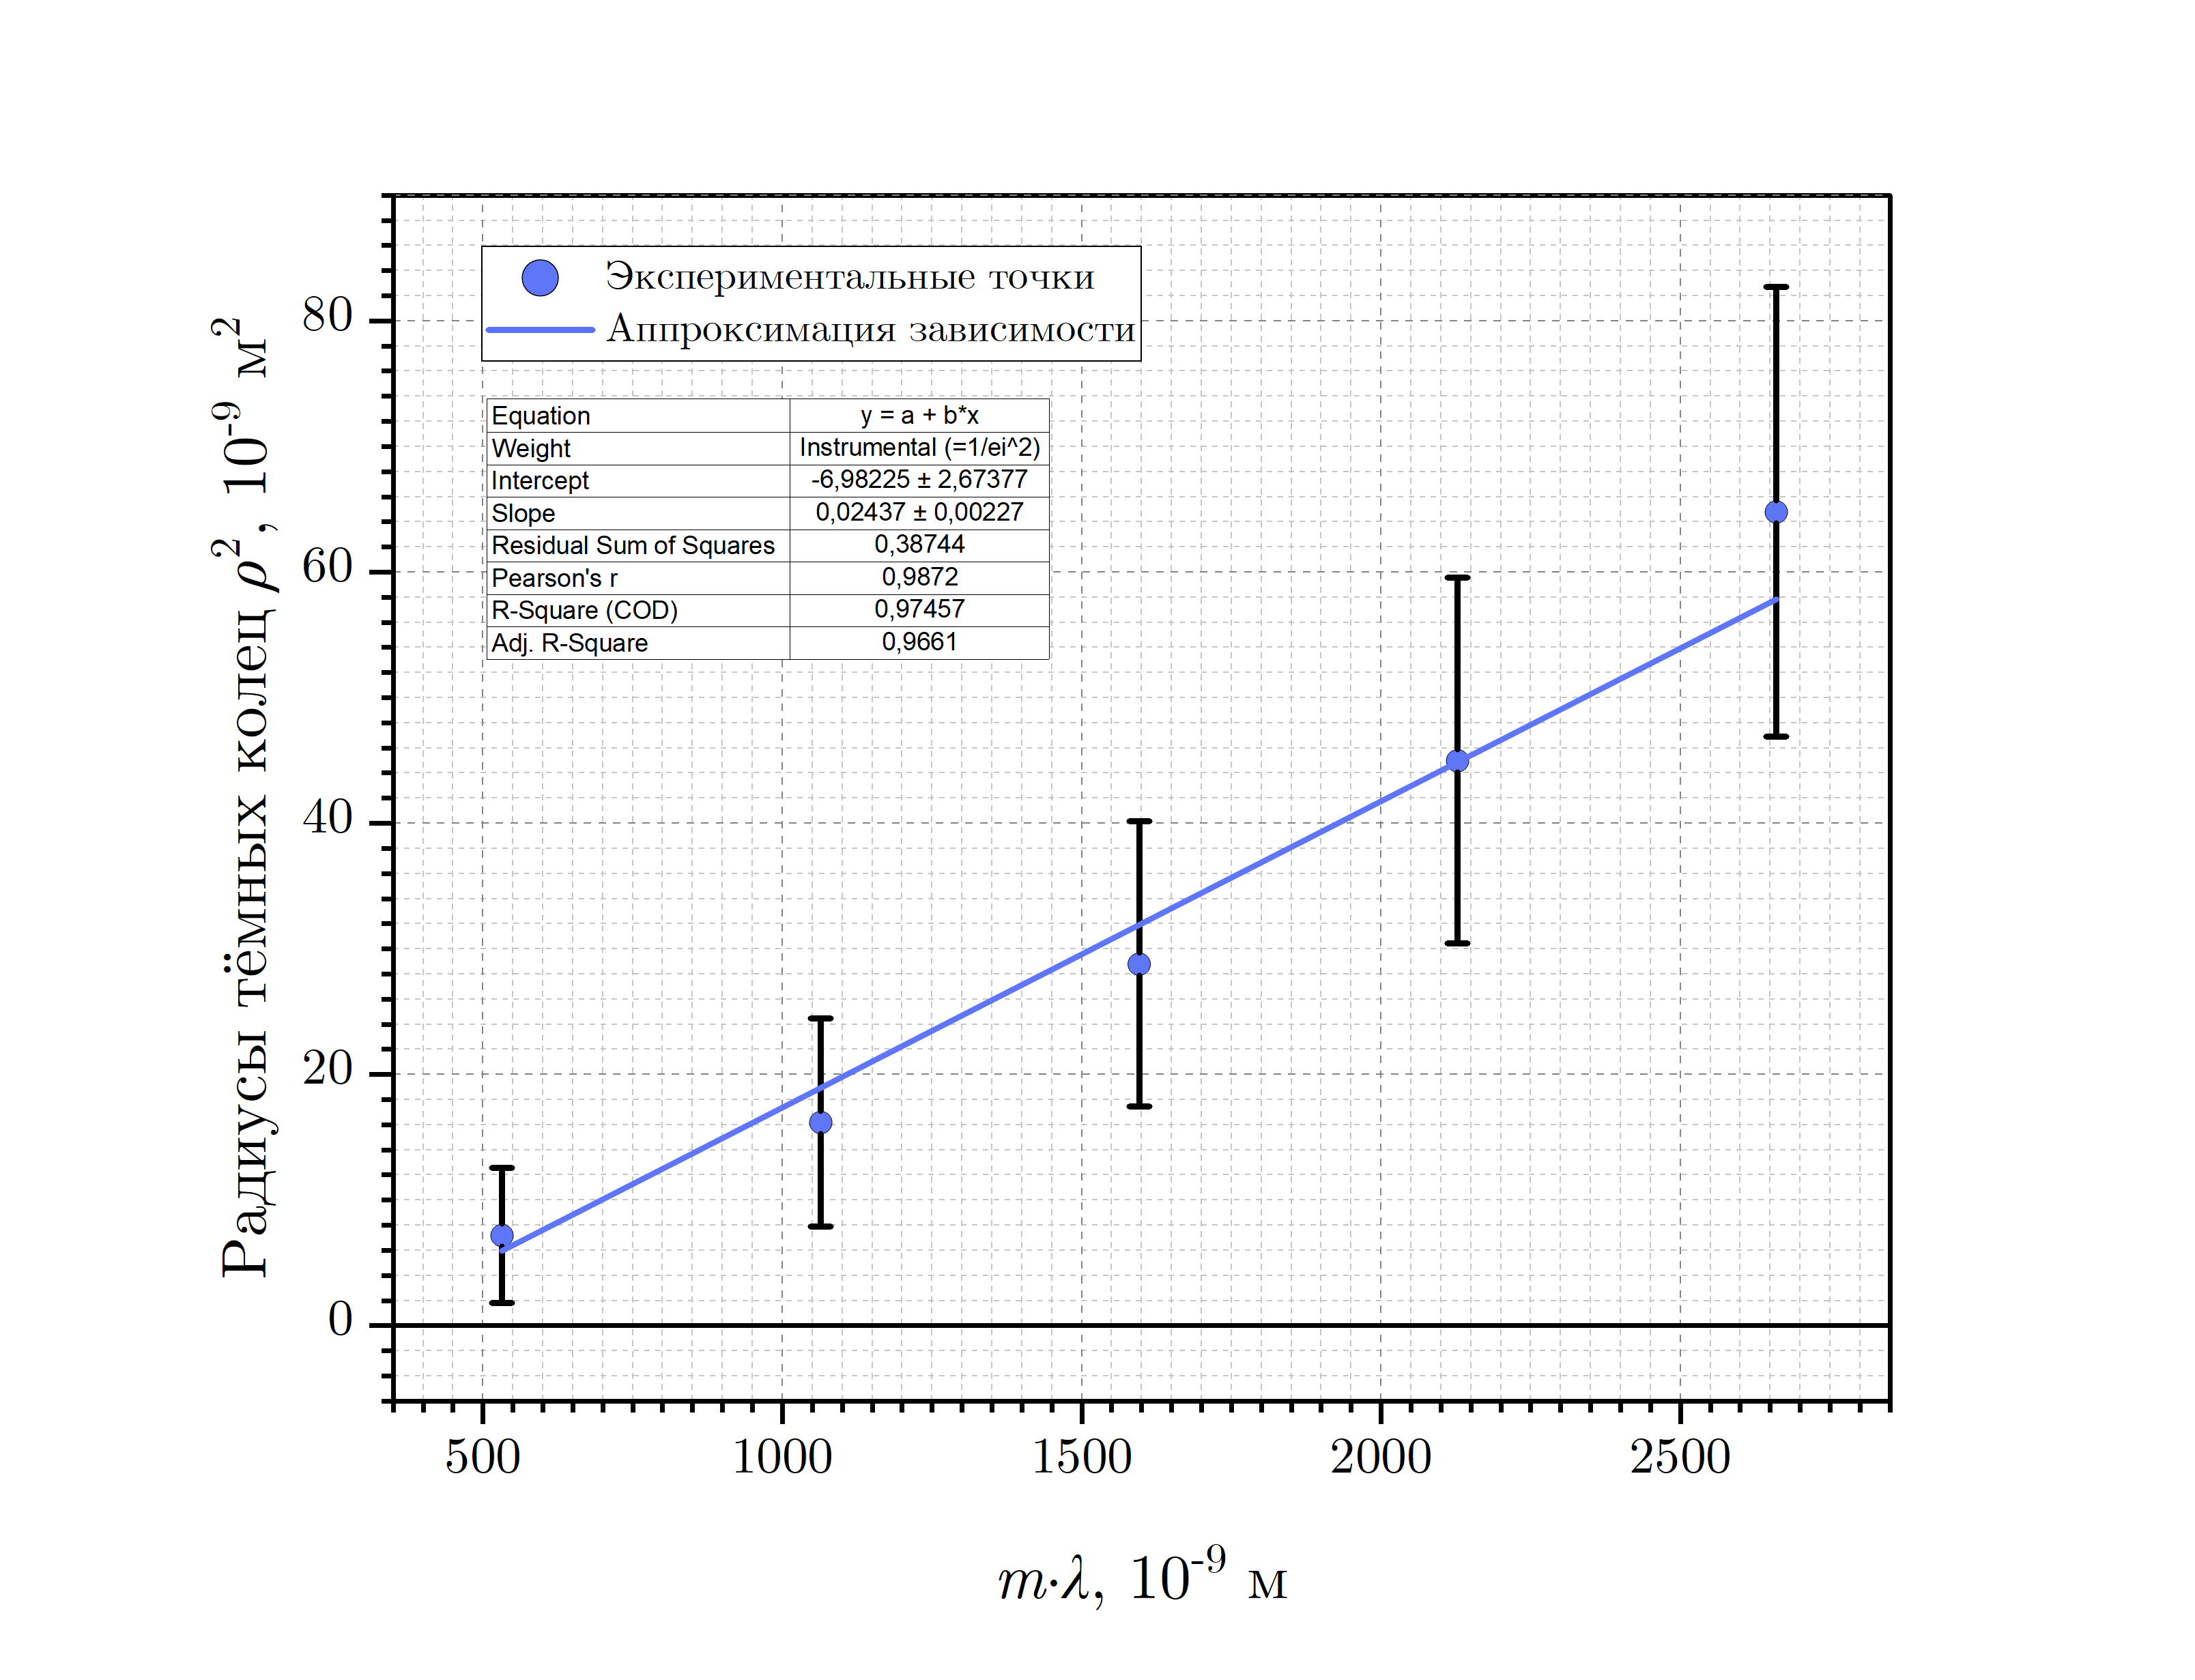
\includegraphics[width = \textwidth]{images/rm_graph.png}
                \caption{График зависимости $\rho^2(m \lambda)$}
            \end{figure}
        
        \column{0.5\textwidth}
            \begin{itemize}
               \item $d = \left( 19 \pm 2 \right) \text{ мм}$ -- расстояние от голограммы до точечного источника
            \end{itemize}
        
        \end{columns}
    \end{frame}

    \begin{frame}{Изучение фокусирующих свойств голограммы}
    \small

    В этой части работы голограмма выполняет роль короткофокусной линзы. В качестве транспаранта - предметная шкала.

    \begin{itemize}
        \item $D' = \left( 2.0 \pm 0.5 \right) \text{ мм}$ -- расстояние между штрихами
        \item $d = f = \frac{D}{D'} b = \left( 30 \pm 10 \right) \text{ мм}$ -- фокусное расстояние голографической линзы (расстояние от точечного источника до голограммы)
    \end{itemize}
       
    \end{frame}

    \section{Изучение характеристик голограммы объёмного предмета}

    \begin{frame}{Изучение мнимого изображения}
    \small
        \begin{columns}
        \column{0.5\textwidth}
        \begin{figure}[H]
            \centering
            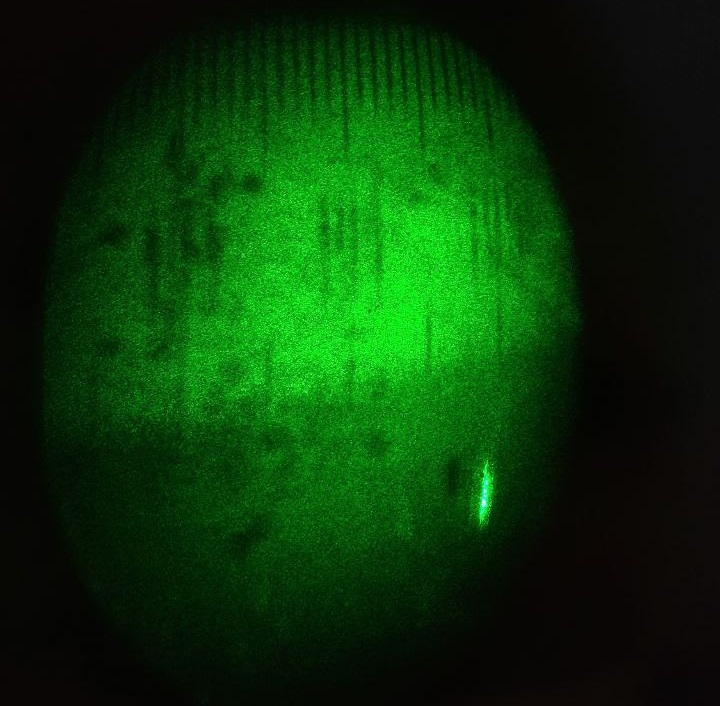
\includegraphics[width = \textwidth]{images/imaginary_image_v.jpg}
            \caption{Голограмма объёмного предмета}
        \end{figure}
        
        \column{0.5\textwidth}
        \begin{itemize}
            \item $\varphi \approx 45^\circ$ -- угол падения опорной волны (угол поворота голограммы)
            \item Изображение предмета восстанавливается по небольшой части голограммы
        \end{itemize}
        \end{columns}
    \end{frame}

    \begin{frame}{Изучение действительного изображения}
    \small
        \begin{columns}
        \column{0.5\textwidth}
        \begin{figure}[H]
            \centering
            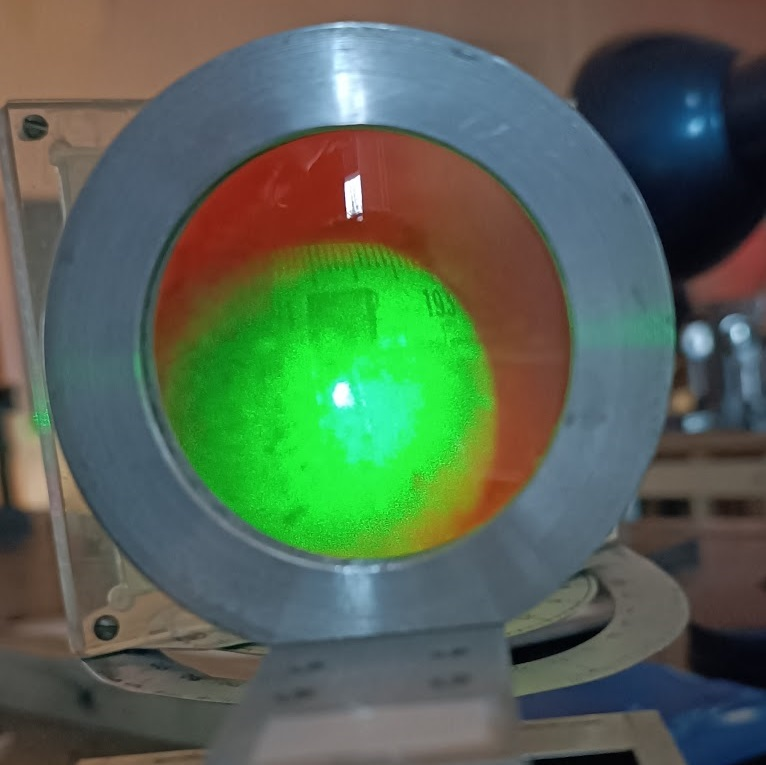
\includegraphics[width = \textwidth]{images/imaginary_image_lens.jpg}
            \caption{Голограмма объёмного предмета}
        \end{figure}
        
        \column{0.5\textwidth}
        \begin{itemize}
            \item Масштаб действительного изображения увеличивается при приближении короткофокусной линзы к голограмме
        \end{itemize}
        \end{columns}
    \end{frame}
    
    \section{Заключение}
    
    \begin{frame}{Выводы}
        \begin{itemize}
            \item Вследствие большой погрешности прямых измерений, вычисление расстояния от точечного источника до голограммы не обладает достаточной точностью
            \item Изображение предмета восстанавливается по небольшой части голограммы
            \item При падении сферической восстанавливающей волны наблюдалось изменение масштабов изображение при перемещении короткофокусной линзы
            \item В случае произвольного предмета интерференционный узор на голограмме можно рассматривать как совокупность зонных кольцевых решёток Габора
        \end{itemize}
    \end{frame}

    \section{Список литературы}
    \begin{frame}{Список литературы}
        \printbibliography
    \end{frame}
    
\end{document}